\documentclass[border=30pt]{standalone}
\usepackage{cyrcam} 
\usepackage{tikz}
\begin{document}
	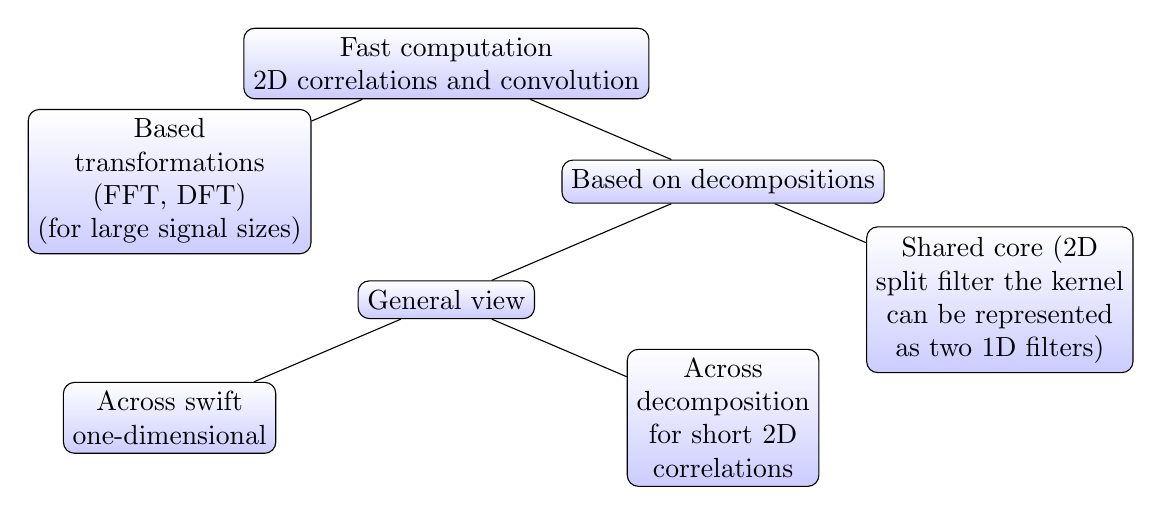
\begin{tikzpicture}[sibling distance=20em,
		every node/.style = {shape=rectangle, rounded corners,
			draw, align=center,
			top color=white, bottom color=blue!20}]]
		\node {Fast computation \\ 2D correlations and convolution}
		child { node {Based \\
				transformations \\
				(FFT, DFT) \\
				(for large signal sizes)} }
		child { node {Based on decompositions}
			child { node {General view}
				child { node {Across swift \\
						one-dimensional} }
				child { node { Across \\
						decomposition \\
						for short 2D \\
						correlations} }
				 }
			child { node {Shared core (2D \\
					split filter the kernel \\ 
					can be represented \\
					as two 1D filters)} } };
	\end{tikzpicture}
\end{document}